\documentclass[10pt, a4paper, onecolumn, oneside, titlepage, openany]{book}

\usepackage[T1]{fontenc}
\usepackage[utf8]{inputenc}
\usepackage{titlesec} % chapter on line with text
\usepackage{fancyhdr}
\usepackage{hyperref}
\hypersetup{
    colorlinks=true,
    linkcolor=blue, %\ref{}
    filecolor=magenta, % \href{run:./file.txt}{File.txt}
    urlcolor=cyan, % \href{http://www.overleaf.com}{Link}
    pdftitle={Cisco CCNA}
    pdfpagemode=FullScreen,
    }
\usepackage{menukeys}
\usepackage{fancyvrb}

% table formatting
\setlength{\arrayrulewidth}{0.5mm} % border
\setlength{\tabcolsep}{18pt} % space from border (X axis)
\renewcommand{\arraystretch}{1.5} % space from border (Y axis)
\usepackage[format=hang,font=small,labelfont=bf]{caption} % bold table caption

% chapter formatting
\renewcommand{\chaptername}{}
\titleformat{\chapter}[hang]{\normalfont\huge\bfseries}{\chaptertitlename\ \thechapter.}{1em}{}

% decorative lines:
\renewcommand{\headrulewidth}{2pt}
\renewcommand{\footrulewidth}{2pt}
\pagestyle{fancy}
\fancyhf{}
    \chead{\leftmark}
    \cfoot{\thepage}
\fancypagestyle{plain}{
\fancyhf{}
    \chead{\leftmark}
    \cfoot{\thepage}
}

% verbatim formatting
\definecolor{device}{RGB}{0, 100, 200}
\definecolor{command}{RGB}{41, 182, 0}
\definecolor{nocommand}{RGB}{222, 0, 0}
\definecolor{showcommand}{RGB}{255, 80, 0}
\definecolor{warncommand}{RGB}{255, 80, 0}
\definecolor{root}{RGB}{222, 0, 0}
\definecolor{user}{RGB}{0, 150, 0}
\definecolor{dir}{RGB}{0, 100, 200}
\definecolor{file}{RGB}{77, 187, 101}
\definecolor{block}{RGB}{255, 80, 0}
\definecolor{comment}{RGB}{0, 182, 182}
\definecolor{background}{RGB}{240, 240, 240}
\renewcommand{\FancyVerbFormatLine}[1]{\colorbox{background}{#1}}


\title{\textbf{Linux Gentoo}}
\author{AISK11}
\date{March 2022}

\begin{document}
\maketitle
\tableofcontents


\chapter{System Info/Requirements}
\section{System Hardware}
\begin{table}[h!]
\centering
\begin{tabular}{|c|c|}
    \hline
    \textbf{Hardware} & \textbf{Value} \\
    \hline
    CPU architecture & amd64\\
    Motherboard & UEFI\\
    WiFi & iwlwifi\\
    GPU & Nvidia\\
    \hline
\end{tabular}
\caption{System hardware overview.}
\label{table:1}
\end{table}


\chapter{Download}
\section{Download Gentoo ISO}
\begin{enumerate}
    \item \textbf{Download Gentoo ISO}
    \begin{itemize}
        \item \textbf{General Gentoo download page:}
\newline \url{https://www.gentoo.org/downloads/}
        \item \textbf{Gentoo files from mirror (image, stage3, signatures):}
\newline \url{https://bouncer.gentoo.org/fetch/root/all/releases/amd64/autobuilds/current-install-amd64-minimal/}
    \end{itemize}
    \item \textbf{Verify download:}
\end{enumerate}

\section{USB preparation}
\begin{enumerate}
    \item \textbf{Unmount USB FS!}
    \item \textbf{Flash image to USB:}
\begin{Verbatim}[commandchars=\\\{\}]
\textcolor{root}{root#} \textcolor{command}{dd} if=<\textcolor{file}{./install-amd64-minimal-<release>.iso}> of=<\textcolor{block}{/dev/sdX}>
[conv=fsync] [bs=4M] [status=progress]
\end{Verbatim}
\end{enumerate}

\section{Boot Live Installer}
\subsection{Secure Boot}
Make sure, that Secure Boot is disabled!
\begin{enumerate}
    \item \textbf{During POST press key to access BIOS/UEFI:}
\newline \href{https://techofide.com/blogs/boot-menu-option-keys-for-all-computers-and-laptops-updated-list-2021-techofide/}{https://techofide.com/blogs/boot-menu-option-keys-for-all-computers-and-laptops-updated-list-2021-techofide/}
    \item \textbf{Disable Secure Boot}
    \item \textbf{Poweroff/Restart}
\end{enumerate}
\subsection{Boot}
\begin{enumerate}
    \item \textbf{Plug in flashed USB}
    \item \textbf{During POST press key to access Boot Menu:}
\newline \href{https://techofide.com/blogs/boot-menu-option-keys-for-all-computers-and-laptops-updated-list-2021-techofide/}{https://techofide.com/blogs/boot-menu-option-keys-for-all-computers-and-laptops-updated-list-2021-techofide/}
    \item \textbf{Select USB entry (UEFI)}
\end{enumerate}


\chapter{Pre-Installation}
\section{Verify UEFI}
\begin{enumerate}
    \item \textbf{UEFI is used if following directory exists:}
\newline \textbf{\textcolor{dir}{/sys/firmware/efi/}}
\end{enumerate}

\section{Check Disk Sectors}
\subsection{Theory}
\begin{itemize}
    \item \textbf{Sector:} smallest unit size on disk. Usually 512 bytes, but some hard disks have 4096.
    \item \textbf{Block:} Allocation size the FS uses. Cannot be smaller than size of the sector. Can be group of sectors (4096b: 8 x 512b sectors).
    \begin{itemize}
        \item \textbf{512b =} good for lot of small files. More blocks = more metadata.
        \item \textbf{4096b =}  good for larger files, less metadata. Waste if there are mostly small files.
    \end{itemize}
\end{itemize}
\subsection{Disk Information}
\begin{itemize}
    \item \textbf{Find disks (block devices):}
\begin{Verbatim}[commandchars=\\\{\}]
\textcolor{user}{user\$} \textcolor{command}{lsblk} [-ap | -apf]
\textcolor{root}{root#} \textcolor{command}{fdisk -l} [\textcolor{block}{/dev/sdX}]
\textcolor{root}{root#} \textcolor{command}{gdisk -l} <\textcolor{block}{/dev/sdX}>
\textcolor{root}{root#} \textcolor{command}{blkid}
\end{Verbatim}
    \item \textbf{Get raw disk info:}
    \begin{itemize}
        \item \textbf{Disk size in bytes:}
\begin{Verbatim}[commandchars=\\\{\}]
\textcolor{root}{root#} \textcolor{command}{blockdev} [-v] --getsize64 <\textcolor{block}{/dev/sdX[Y]}>
\end{Verbatim}
    \item \textbf{Disk block size in bytes:}
\begin{Verbatim}[commandchars=\\\{\}]
\textcolor{root}{root#} \textcolor{command}{blockdev} [-v] --getbsz <\textcolor{block}{/dev/sdX[Y]}>
\end{Verbatim}
    \item \textbf{Check if disk is readonly (1 = ro, 0 = rw):}
\begin{Verbatim}[commandchars=\\\{\}]
\textcolor{root}{root#} \textcolor{command}{blockdev} [-v] --getro <\textcolor{block}{/dev/sdX[Y]}>
\end{Verbatim}
    \end{itemize}
    \item \textbf{See partitions:}
\begin{Verbatim}[commandchars=\\\{\}]
\textcolor{root}{root#} \textcolor{command}{parted} -s <\textcolor{block}{/dev/sdX}> (p)rint [free]
\end{Verbatim}
\end{itemize}
\subsection{Check Disk for bad sectors}
\begin{enumerate}
    \item \textbf{Unmount FS!}
    \item \textbf{Check disk for bad blocks:}
\begin{Verbatim}[commandchars=\\\{\}]
\textcolor{root}{root#} \textcolor{command}{badblocks} [-b 4096] [-w [-t 0xaa]] [-v] [-s]
<\textcolor{block}{/dev/sdX[Y]}> | \textcolor{command}{tee} -a <\textcolor{file}{OUTPUT_FILE}>
\end{Verbatim}
\end{enumerate}

\section{Connect to the internet}
\begin{itemize}
    \item \textbf{Ethernet}

    \item \textbf{WiFi}
\end{itemize}


\chapter{Installation}
\section{Disk Partitioning}
\subsection{Partition Table}
\begin{enumerate}
    \item \textbf{Unmount FS!}
    \item \textbf{Create GPT partition table:}
\begin{Verbatim}[commandchars=\\\{\}]
\textcolor{root}{root#} \textcolor{command}{parted} -s <\textcolor{block}{/dev/sdX}> mktable gpt
\end{Verbatim}
\end{enumerate}
\subsection{Basic Partitions}
\begin{enumerate}
    \item \textbf{Enter cfdisk:}
\begin{Verbatim}[commandchars=\\\{\}]
\textcolor{root}{root#} \textcolor{command}{cfdisk} <\textcolor{block}{/dev/sdX}>
\end{Verbatim}
    \item \textbf{Create EFI partition (recommended 550 MiB):}
\begin{Verbatim}[commandchars=\\\{\}]
\textcolor{root}{cfdisk>} \textcolor{command}{n}
\textcolor{root}{cfdisk>} \textcolor{command}{550MiB}
\textcolor{root}{cfdisk>} \textcolor{command}{t}
\textcolor{root}{cfdisk>} \textcolor{command}{EFI System}
\end{Verbatim}
    \item \textbf{Create encrypted partition:}
\begin{Verbatim}[commandchars=\\\{\}]
\textcolor{root}{cfdisk>} \textcolor{command}{n}
\textcolor{root}{cfdisk>} \textcolor{command}{ } (Enter)
\end{Verbatim}
    \item \textbf{Write changes:}
\begin{Verbatim}[commandchars=\\\{\}]
\textcolor{root}{cfdisk>} \textcolor{command}{W}
\textcolor{root}{cfdisk>} \textcolor{command}{yes}
\end{Verbatim}
    \item \textbf{Quic cfdisk:}
\begin{Verbatim}[commandchars=\\\{\}]
\textcolor{root}{cfdisk>} \textcolor{command}{Q}
\end{Verbatim}
    \item \textbf{Name partitions:}
\begin{Verbatim}[commandchars=\\\{\}]
\textcolor{root}{root#} \textcolor{command}{parted} -s <\textcolor{block}{/dev/sdX}> name 1 ESP
\textcolor{root}{root#} \textcolor{command}{parted} -s <\textcolor{block}{/dev/sdX}> name 2 LUKS
\end{Verbatim}
    \item \textbf{Format partitions:}
    \begin{enumerate}
        \item \textbf{ESP:}
\begin{Verbatim}[commandchars=\\\{\}]
\textcolor{root}{root#} \textcolor{command}{mkfs.fat} -F 32 <\textcolor{block}{/dev/sdX1}>
\textcolor{root}{root#} \textcolor{command}{fatlabel} <\textcolor{block}{/dev/sdX1}> <ESP>
\end{Verbatim}
        \item \textbf{LUKS:}
\begin{Verbatim}[commandchars=\\\{\}]
\textcolor{root}{root#} \textcolor{command}{cryptsetup} luksFormat --label <LUKS> <\textcolor{block}{/dev/sdX2}>
> YES
> <PASSWORD>
> <PASSWORD (VERIFY)>
\end{Verbatim}
    \end{enumerate}
\end{enumerate}
    \subsection{Advanced LUKS stuff}
\begin{itemize}
    \item \textbf{Open LUKS:}
\begin{Verbatim}[commandchars=\\\{\}]
\textcolor{root}{root#} \textcolor{command}{cryptsetup} open --type luks <\textcolor{block}{/dev/sdX2}> <luks>
> <PASSWORD>
\end{Verbatim}
    \item \textbf{Close LUKS:}
\begin{Verbatim}[commandchars=\\\{\}]
\textcolor{root}{root#} \textcolor{command}{cryptsetup} close <luks>
\end{Verbatim}
    \item \textbf{LUKS header:}
    \begin{enumerate}
        \item \textbf{See LUKS header:}
\begin{Verbatim}[commandchars=\\\{\}]
\textcolor{root}{root#} \textcolor{command}{cryptsetup} luksDump <\textcolor{block}{/dev/sdX2}>
\end{Verbatim}
        \item \textbf{Make LUKS header backup:}
\begin{Verbatim}[commandchars=\\\{\}]
\textcolor{root}{root#} \textcolor{command}{cryptsetup} luksHeaderBackup <\textcolor{block}{/dev/sdX2}>
--header-backup-file <\textcolor{file}{FILE}>
\end{Verbatim}
        \item \textbf{Destroy LUKS header:}
\begin{Verbatim}[commandchars=\\\{\}]
\textcolor{root}{root#} \textcolor{command}{cryptsetup} luksErase <\textcolor{block}{/dev/sdX2}>
> YES
\end{Verbatim}
        \item \textbf{Restore LUKS header:}
\begin{Verbatim}[commandchars=\\\{\}]
\textcolor{root}{root#} \textcolor{command}{cryptsetup} luksHeaderRestore <\textcolor{block}{/dev/sdX2}>
--header-backup-file <\textcolor{file}{FILE}>
> YES
\end{Verbatim}
    \end{enumerate}
\end{itemize}
\subsection{Encrypted LVM Partition}
\begin{figure}[ht]
    \begin{center}
        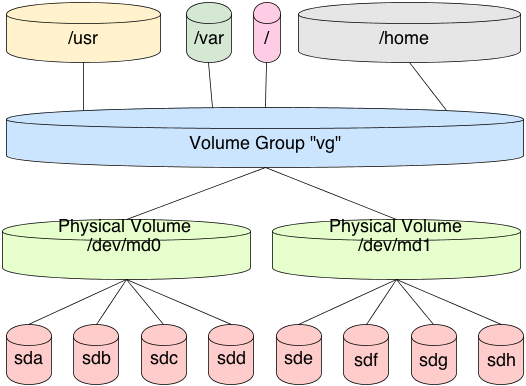
\includegraphics[width=115mm]{./src/images/lvm.png}
        \caption{LVM structure.}
        \label{fig:1}
    \end{center}
\end{figure}
\begin{enumerate}
    \item \textbf{Open encrypted partition:}
\begin{Verbatim}[commandchars=\\\{\}]
\textcolor{root}{root#} \textcolor{command}{cryptsetup} open --type luks <\textcolor{block}{/dev/sdX2}> <luks_lvm>
> <PASSWORD>
\end{Verbatim}
    \item \textbf{Create LVM Physical Volume:}
\begin{Verbatim}[commandchars=\\\{\}]
\textcolor{root}{root#} \textcolor{command}{lvm} pvcreate <\textcolor{block}{/dev/mapper/luks_lvm}>
\end{Verbatim}
    \item \textbf{Create LVM Volume Group:}
\begin{Verbatim}[commandchars=\\\{\}]
\textcolor{root}{root#} \textcolor{command}{lvm} vgcreate <vg0> <\textcolor{block}{/dev/mapper/luks_lvm}>
\end{Verbatim}
    \item \textbf{Create LVM Logical Volumes:}
    \begin{enumerate}
        \item \textbf{Root Logical Volume:}
\begin{Verbatim}[commandchars=\\\{\}]
\textcolor{root}{root#} \textcolor{command}{lvm} lvcreate -l 100\%FREE -n <root> <vg0>
\end{Verbatim}
    \end{enumerate}
    \item \textbf{Verify LVM}
    \begin{itemize}
        \item \textbf{Check LVM Physical Volumes:}
\begin{Verbatim}[commandchars=\\\{\}]
\textcolor{root}{root#} \textcolor{command}{lvm} pvdisplay
\end{Verbatim}
        \item \textbf{Check LVM Volume Groups:}
\begin{Verbatim}[commandchars=\\\{\}]
\textcolor{root}{root#} \textcolor{command}{lvm} vgdisplay [vg0]
\end{Verbatim}
        \item \textbf{Check LVM Logical Volumes:}
\begin{Verbatim}[commandchars=\\\{\}]
\textcolor{root}{root#} \textcolor{command}{lvm} lvdisplay
\end{Verbatim}
    \end{itemize}
    \item \textbf{Format LVM Logical Volumes:}
    \begin{enumerate}
        \item \textbf{Root Partition:}
\begin{Verbatim}[commandchars=\\\{\}]
\textcolor{root}{root#} \textcolor{command}{mkfs.btrfs} <\textcolor{block}{/dev/vg0/root}>
\textcolor{root}{root#} \textcolor{command}{btrfs} filesystem label <\textcolor{block}{/dev/vg0/root}> <LVM_ROOT>
\end{Verbatim}
    \end{enumerate}
\end{enumerate}

\section{Gentoo Installation}
\begin{enumerate}
    \item \textbf{Mount Gentoo:}
\begin{Verbatim}[commandchars=\\\{\}]
\textcolor{root}{root#} \textcolor{command}{mount} <\textcolor{block}{/dev/mapper/vg0-root}> \textcolor{dir}{/mnt/gentoo}
\end{Verbatim}


\end{enumerate}

\end{document}
